\documentclass[11pt, a4paper]{article}
\usepackage{multirow}
\usepackage{enumerate}
\usepackage{geometry}
\geometry{left=2.5cm,right=2.5cm,top=2.5cm,bottom=2.5cm}
%\usepackage{minted}
\usepackage[slantfont,boldfont]{xeCJK}
\setCJKmainfont{SimSun}
\usepackage{indentfirst}
\usepackage{float}
\setlength{\parindent}{2em}
\setCJKmonofont{SimHei}
\input zhwinfonts
\renewcommand\figurename{图}
\renewcommand\tablename{表}
\renewcommand\contentsname{\centering 目录}

\begin{document}
\title{{\bf\Huge UpBit与其他位图索引的不足} \\[2ex]{\huge 《算法设计与分析》课程第三次作业}}
  \author{计算机科学与技术学院\\马玉坤\\1150310618}
  \date{2017年5月9日}
  \maketitle

  \emph{在当今这个数据爆炸的时代,数据仓库的地位越来越重要。在众多数据仓库的实现方案中,位图索引被广泛应用。UpBit是一种创新的位图索引,对于需要少量修改、大量查询的场景十分有效。本文由UpBit效率的瓶颈出发,从修改操作角度,对若干位图索引的不足进行了说明。}\\
  {\bf 关键字:}位图索引,数据仓库,位图编码

  %% \tableofcontents

  \section{背景介绍}

  \subsection{位图索引}

  位图索引 (Bitmap Index)由P’ONeil在1987年提出,并在一个商用数据库系统Model 204上首次应用。在数据库中,无论是用于科研用途,还是商业用途,位图索引都被广泛应用。近年来,随着互联网以及计算机硬件的发展,科研与商业中所使用的数据量不断增大,这也对位图索引提出了更高的要求。近年来,位图索引领域有许多研究成果,其中UpBit\cite{art1}是一个新近提出的在内存中使用的支持修改操作的效率较高的位图索引。

  \subsection{Upbit}

  UpBit对每个属性都使用了一个更新向量(Update Bitvector,UB)。每一个属性的位向量,用两个位向量经“位异或”计算得出,这两个位向量分别为值向量 (Value Bitvector,VB)与更新向量 (Update Bitvector,UB)。\cite{art1}

  由于每一个属性的位向量用两个位向量经“位异或”计算得出。所以无论我们修改UB或者VB,都相当于对属性进行修改。在每次修改操作时,我们直接修改UB的值。如图\ref{fig:upbit},当我们想要把第二行的值从20修改为10,只需要把属性20对应的$UB_i$取反(从0变为1或者从1变为0),然后把属性10对应的$UB_i$取反。

  \begin{figure}[H]
    \begin{center}
      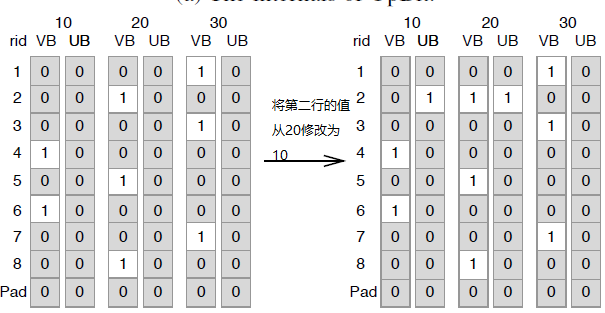
\includegraphics[width=5.5in]{upbit.png}
      \caption{Upbit图解}\label{fig:upbit}
    \end{center}
  \end{figure}

  \subsubsection{定时维护更新向量}

  当某个属性的UB的修改次数达到一定阈值时,我们将该属性的VB与UB做异或操作,将结果保存到VB中,然后将UB设为全0的向量,这便是对UB的维护。这样的维护可以保证随着修改操作积累,查询的效率仍然可以很快。

  \subsubsection{维护向量的分块指针}

  同时,UpBit还使用了第二种关键的提高效率的方法——块指针 (Fence Pointers)。当我们对某一行的值进行修改时,首先就需要找到这一行修改前的值。在寻找这一行修改前的值的过程中,我们需要在每一个属性的压缩后的UB和VB中查询这一行对应的二进制位的值。如何在压缩后的位向量中,快速找到第i位的值,是一个与效率关系极大的问题。块指针的思想是:将未压缩前的位向量按下标分为若干连续的块,每一块的块大小都接近g (g是人为给定的值)。对于每个位向量,维护每一块的起始位置对应的行在压缩后的位向量中的位置,就可以在$O(g+\log N/g)$的时间复杂度内快速在每个压缩后位向量中找到任意一行的位置,并可在$O(N/g)$的时间复杂度内维护修改后位向量的块指针。

  \section{若干位图索引的不足(从对位图索引进行修改操作的角度)}

  \subsection{UpBit的效率瓶颈}

  \subsubsection{找到某一行的当前值}

  实际上,在UpBit的实现中,当想要将一行从当前值修改为新值时,如图\ref{fig:get_value},要对每一个值对应的位向量进行查询,效率较低。比如值域大小为10,那么最坏情况下每次获得某一行的值,就需要对20个位向量进行查询(10个UB和10个VB)。实际上,在作者的实验中,当值域大小为100时,这个操作就已经消耗了了整个修改流程的93\%时间。

  因此,在进行修改操作时,UpBit的效率瓶颈在于找到某一行的值。那么如何改进呢?下次作业详细说。

  \begin{figure}[H]
    \begin{center}
      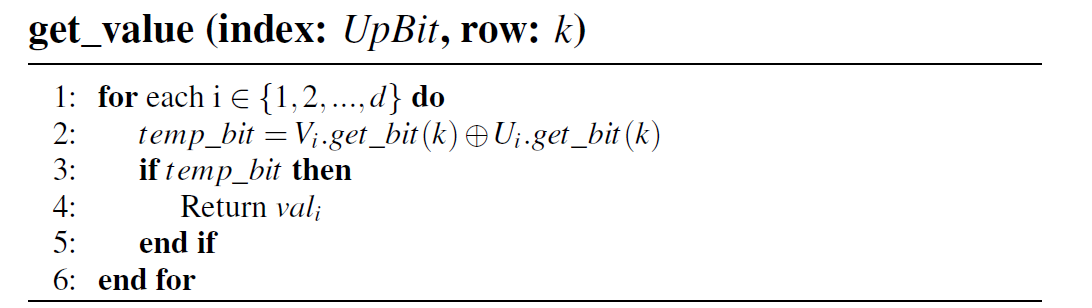
\includegraphics[width=5.5in]{get_value.png}
      \caption{UpBit中获取某一行的当前值算法}\label{fig:get_value}
    \end{center}
  \end{figure}

  \subsubsection{范围查询}

  UpBit对于单值查询(形如$value = x$)的效率是非常高的,但是却不能很快的进行范围查询(形如$value \leq x$)。那么,能不能使用其他位图索引,与UpBit结合,使得UpBit能够较为高效地进行范围查询?换句话说,有没有比较优秀的位图索引,支持单值修改,范围查询?从本人查阅的资料来看,目前并没有比较有效的方法。详见\ref{section:other_bitmaps}。

  \subsection{其他位图索引的效率瓶颈} \label{section:other_bitmaps}

  \subsubsection{单值编码位图索引}

  单值编码位图索引即为最朴素的位图索引(不考虑压缩算法)。显而易见,对于单值修改操作速度较快,但是找到某一行的当前值与范围查询效率较低,最坏需要查询所有位向量。

  \subsubsection{范围编码位图索引}

  能够较快地完成范围查询的位图索引有“范围编码位图索引”\footnote{范围编码位图索引由$m-1$个位向量$\{B_{m-2}, B_{m-3}, \ldots, B_1,  B_0\}$组成, 其中 $B_j$ 对应于属性值 $j$, 当且仅当 $t_i.A \le j$ 时,$B_j[i] =1$。范围编码位图索引中, 每一位图向量代表所有小于等于对应值的索引值。\cite{art3}}。然而遗憾的是,范围编码位图索引并不能较快地完成单值修改操作。对每一个单值修改,最坏情况下要修改所有的位向量。

  \subsubsection{分段位图索引}

  分段位图索引\footnote{分段位图索引由 Chan 和 I oannidis 提出,它将属性值用$r$进制表示。 在$r$进制中, 0到$m - 1$之间的每一个值$x$可以用长度为$e$的数字序列 ($x_{e-1}, …, x1, x0$) 表示, 其中 $e =「\log_m{r}」$、$0≤x_e, …, x_1 , x_0 <r$、$x = x_{e - 1} *r^{e-1} +…, + x_1 *r + x_0$。$e$位数字序列可以看成是$e$个列的值组成的, 相应的A列可划分成 e个子列$A_{e-1}, …, A_1, A_0$。 分段位图索引就是分别为每一个子列建立位图索引, 子列索引称为称为元索引, r为索引的基。 对于每一个元索引可以使用等值编码位图索引或范围编码位图索引。}是一种位向量数目较少的位图索引,然而,同样,在最坏情况下,对于单值修改操作,要修改所有的位向量(但需要位向量个数大大减少了,约为$O(k\log_k{d})$数量级,其中k为基大小,d为值域大小)。尽管,但是单值修改较快,但是范围查询比范围编码位图索引慢。然而总体效率仍然不优秀。

\renewcommand\refname{参考文献}
\begin{thebibliography}{99}
\bibitem{art1}Athanassoulis M, Yan Z, Idreos S. UpBit: Scalable In-Memory Updatable Bitmap Indexing[C]//Proceedings of the 2016 International Conference on Management of Data. ACM, 2016: 1319-1332.
\bibitem{art2}Canahuate G, Gibas M, Ferhatosmanoglu H. Update conscious bitmap indices[C]//Scientific and Statistical Database Management, 2007. SSBDM'07. 19th International Conference on. IEEE, 2007: 15-15.
\bibitem{art3}程鹏. 位图索引技术及其研究综述[J]. 科技信息, 2010 (26): 134-135.
\bibitem{art4}Wu K, Ahern S, Bethel E W, et al. FastBit: interactively searching massive data[C]//Journal of Physics: Conference Series. IOP Publishing, 2009, 180(1): 012053.
\bibitem{art5}Wu K, Otoo E J, Shoshani A. Compressing bitmap indexes for faster search operations[C]//Scientific and Statistical Database Management, 2002. Proceedings. 14th International Conference on. IEEE, 2002: 99-108.
\bibitem{art6}Madhu B. Multi-level and Multi-component Bitmap Encoding for Efficient Search Operations[J]. Database Systems Journal, 2012, III(4):47-60.

\end{thebibliography}

\end{document}
